\documentclass[linenumbers, RNAAS, trackchanges]{aastex631}

\usepackage[utf8]{inputenc}
\usepackage{hyperref}           % hrefs
\usepackage{natbib}             % for bibliography
\usepackage{float}              % figure positioning
\usepackage{svg}                % used for SVG images
\usepackage{graphicx}           % used for non-SVG images
\usepackage{amsmath}
\usepackage{parskip}


% Search Query Metadata
\shorttitle{Logistic Map}
%\shortauthors{Nguyen & Vu}

% Hyperlink setup
\hypersetup{
colorlinks=true,
linkcolor=blue,
urlcolor=blue
}

\begin{document}
\title{Bifurcation and Chaos in the Logistic Map}
% [] is for ORCiD
%\correspondingauthor{Main Author}
%\email{author1@email.com, author2@email.com, author3@email.com}
\author{Lily Nguyen}
\affiliation{Department of Physics, The University of Texas at Austin\\
Austin, TX 78712, USA}

\author{Raymond Vu}
\affiliation{Department of ---, The University of Texas at Austin\\
Austin, TX 78712, USA}


% 250 word limit for abstract
\begin{abstract}
\noindent The logistic map is a simple nonlinear difference equation that displays
various behaviors ranging from stable fixed points to periodic oscillations
and chaotic dynamics. In this project, we generated the bifurcation
diagram of the logistic map over the parameter range $2.4< \mu < 4.0$. To reduce
dependence on initial conditions, we followed the standard approach of discarding 
transient iterations and recording the long-term dynamics of $x$
for each $\mu$. The resulting diagram illustrates the progression from
stability to successive period-doubling behavior and the eventual onset of
chaos. The transition occurred near $\mu\approx3.57$, consistent
with the universal period-doubling scenario first described by Feigenbaum \cite{feig}
and later confirmed in numerical studies \cite{chen}. Overall, 
our results align with the mathematical analysis of the logistic map 
\cite{bubolo} and highlight the importance of visualization for understanding
nonlinear systems \cite{boeing}.

\end{abstract}

% Use astrothesaurus numbers in place of num
\keywords{logistic map --- bifurcation diagram --- nonlinear dynamics --- 
chaos theory --- period-doubling bifurcation}


\section{Introduction} \label{sec:intro}

The concept of logistic growth was first introduced by Pierre-François
Verhulst in the 19th century to describe how populations stabilize as they 
approach a maximum carrying capacity \cite{sch}. Although not widely
recognized at the time, his work laid the foundation for later studies of
population dynamics and mathematical modeling.

The modern study of chaos developed much later in the 20th century.
Edward Lorenz, often described as the father of chaos theory, found that
small changes of initial conditions in a simple model of atmospheric convection
could lead to completely different outcomes, making long-term weather
prediction fundamentally impossible \cite{boeing}.

In 1976, Robert May showed that the discrete logistic map, despite its
simplicity, could exhibit oscillations and even chaotic behavior \cite{may}.
Mitchell Feigenbaum later demonstrated that this transition to chaos follows
a period-doubling route, with bifurcations accumulating near $\mu\approx 3.57$
\cite{feig}. Together, these discoveries established the
logistic map as a central model in chaos theory.

Today, the logistic map remains a key tool in nonlinear dynamics.
Its mathematical structure has been studied in detail \cite{bubolo}, and its
bifurcation diagram provides a clear visualization of how order gives way to
chaos \cite{boeing}. As such, the logistic map continues to demonstrate how
simple deterministic rules can generate complex and unpredictable behavior.


\section{Data and Observations} \label{sec:data}

The logistic map is a nonlinear recurrence relation defined by

\begin{equation}
    x_{n+1}=\mu x_n(1-x_n)
\end{equation}

where $0<x_n<1$ is the normalized state variable at the iteration $n$ and $\mu$
is the control parameter with $0<\mu<4$. The goal of this project is to
generate the bifurcation diagram of the logistic map for the parameter range
$2.4\leq\mu\leq4$ to study the transition from stability to chaos. The diagram
shows the long-term values of $x_n$ for each $\mu$ after discarding transient
behavior, revealing fixed points, periodic oscillations, and chaotic dynamics.

To compute the diagram, we varied $\mu$ uniformly between $2.4$ and $4.0$ with
a resolution of 1000 distinct values. For each $\mu$, we initialized the map
with $x_0=0.5$ and iterated $400$ times. We discarded the first $200$
iterations as transients and recorded the final $200$ iterations to represent
long-term behavior. We binned the results to produce a clear density plot of the
bifurcation diagram. The resulting figure (Figure \ref{fig:bifurcation})
displays the bifurcation diagram of the logistic map. Stable fixed points
appear at low values of $\mu$, followed by successive period-doubling
bifurcations, and eventually the onset of chaos near $\mu\approx3.57$.

\begin{figure}[H]
    \centering
    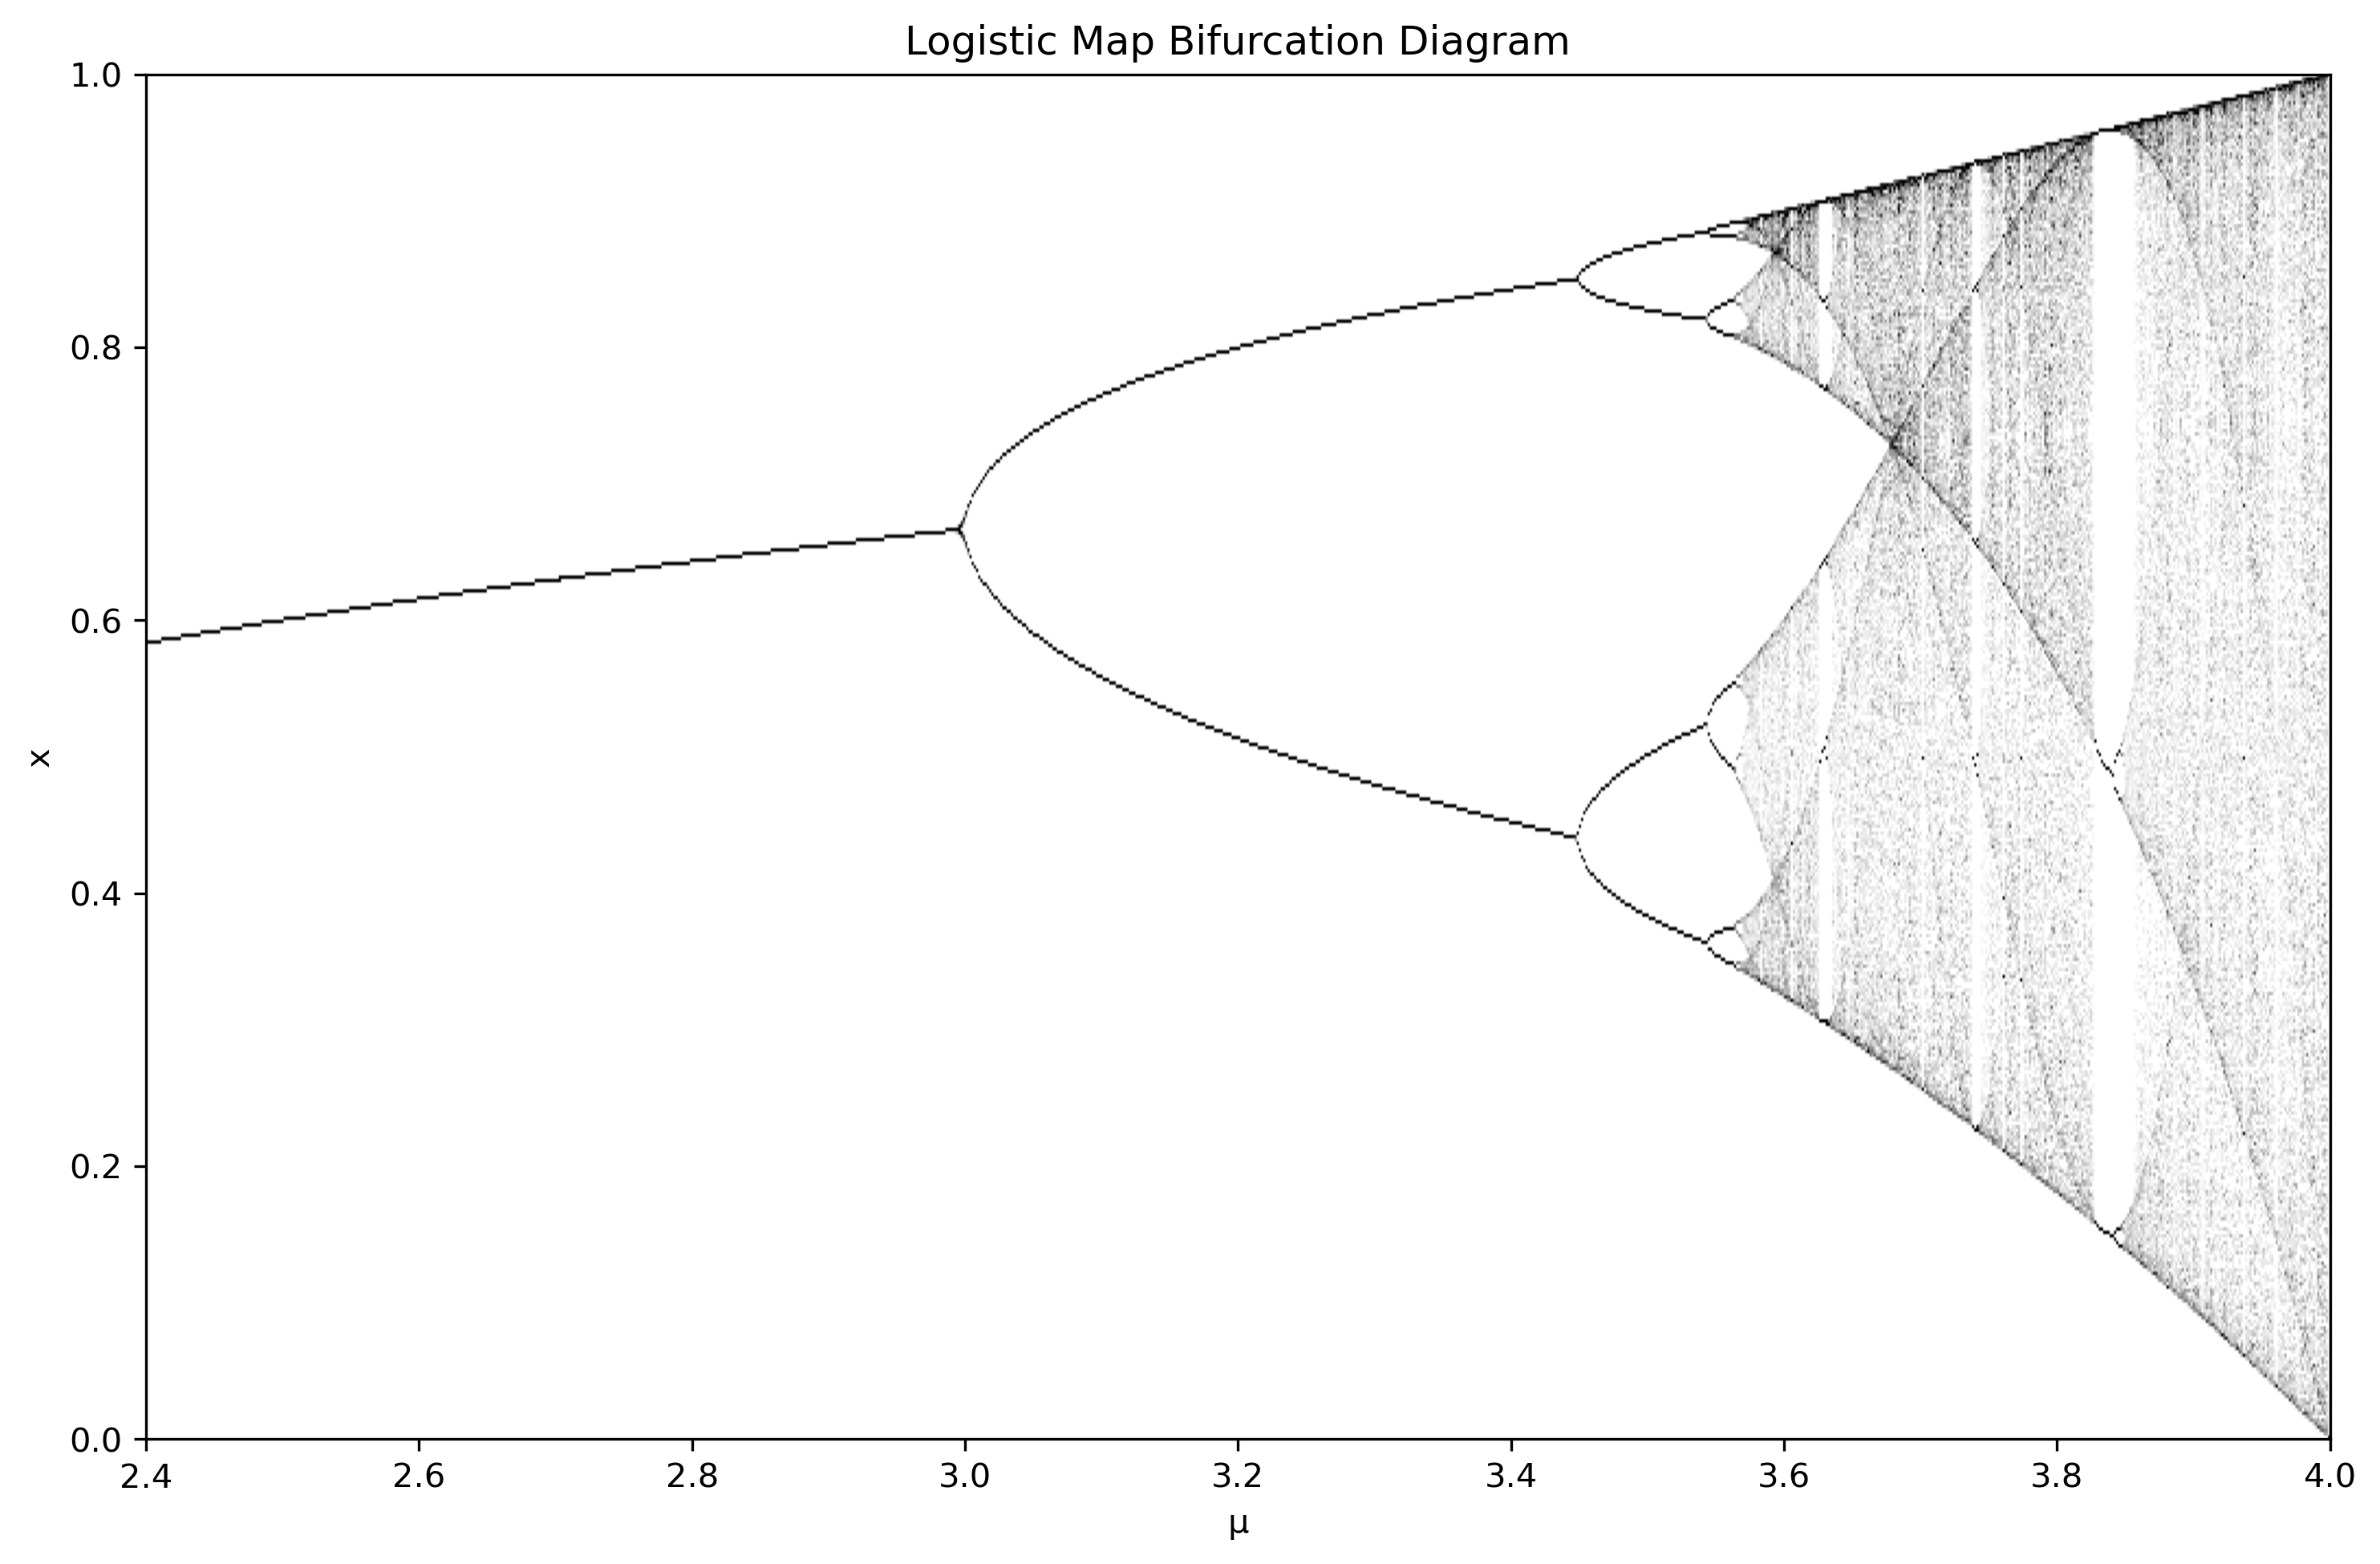
\includegraphics[width=0.65\linewidth]{bifurcation.png}
    \caption{The logistic map bifurcation diagram for $2.4\leq \mu \leq 4.0$. Stable fixed points exist for low values of $\mu$, followed by successive period-doubling bifurcations that lead to chaotic behavior.}
    \label{fig:bifurcation}
\end{figure}


\section{Results} \label{sec:results}
The bifurcation diagram generated for $2.4\leq\mu\leq4.0$ illustrates the
transition from stability to chaos in the logistic map. For small values of
$\mu$, the system converges to a stable fixed point. As $\mu$ increases beyond
$\mu\approx3.0$, the fixed point becomes unstable through a period-doubling
bifurcation, leading to oscillations of period two. Further increases in $\mu$
cause successive period doublings, with period four, eight, and higher powers
of two.

These bifurcations accumulate near $\mu\approx3.57$, the onset of chaos
\cite{feig, chen}. Within the chaotic region, the diagram also reveals
windows of periodicity, demonstrating that ordered behavior can re-emerge
even within chaos.

Potential sources of error include the finite resolution in $\mu$, which limits
how precisely the bifurcation points can be located, as well as the limited
number of iterations used, which constrains the model's accuracy in chaotic
regions. Despite these limitations, the bifurcation diagram reproduced the
expected features with enough clarity to capture the route from stability
to chaos.

\section{Summary and Conclusion} \label{sec:summary}
This project demonstrated the transition from stability to chaos in the
logistic map by generating its bifurcation diagram. Our results align with
theoretical predictions, showing successive period doublings and the onset of
chaos near $\mu\approx3.57$. Our findings confirm the logistic map as an
accepted model for illustrating how a deterministic equation can generate highly
complex and unpredictable behavior.

Beyond reproducing known features, this project highlights the value of
visualization in understanding nonlinear dynamics. Future work may include
calculating the Lyapunov exponent to quantify chaos or comparing the logistic
map with continuous systems such as the Lorenz attractor. Investigating the 
fractal geometry could also deepen our understanding of the the scaling
behavior found in chaotic systems.


\subsection{Acknowledgements}
We thank Professor Mitra for his guidance and instruction throughout the course,
as well as the teaching assistants for their helpful feedback. We also
acknowledge the Department of Physics for providing the broader academic
foundation to support this work. This paper was completed as part of the 
requirements for C S 323E: Elements of Scientific Computing at the University
of Texas at Austin.

\newpage
\bibliographystyle{aasjournal}
\bibliography{refs}

\end{document}
